\section*{2. What Each Lane Was Trying To Do}

\rowcolors{2}{white}{warmbg}
\begin{table}[H]
    \centering
    \small
    \begin{tabularx}{\linewidth}{>{\bfseries}p{0.18\linewidth} >{\raggedright\arraybackslash}p{0.24\linewidth} >{\raggedright\arraybackslash}p{0.24\linewidth} X}
        \rowcolor{tealaccent!14}
        Lane & Core idea & Why it was tried & Verdict \\
        Early boosted trees & LightGBM, XGBoost, ExtraTrees, and simple blends on a shared holdout split & Fast way to beat the template and check whether the local validation scheme was trustworthy & It worked well enough to calibrate Kaggle quickly and became the foundation for the next families. \\
        Poly parallel + MPS & Broader engineered features plus an extra MPS-supported branch & Test whether wider but still readable feature work could move the score before deeper refactors & It improved on the baseline and made branch-first thinking natural. \\
        Overnight ensemble & Tuned XGB, LGB, CatBoost, ExtraTrees, MPS, and a learned combiner & Build one serious tabular family instead of many half-related scripts & This became the cleanest strong lane and later the public-facing path. \\
        Target-stats family & OOF target statistics, stronger pruning, and richer tabular blending & Push the classical branch as far as possible before giving up on feature-side work & This became the main upstream source for the strongest local hybrids. \\
        Neural and meta layers & Wide-deep, residual MLP, classifier-only blend, meta stack, and weighted blend & Check whether neural or meta layers could squeeze more value out of strong tabular predictions & Light meta layers helped. Fully replacing the tabular core usually did not. \\
        Professor lane & Broader feature factory, stronger missingness features, classical screening, and GA-style refinement after pruning & Systematically test the professor's suggestions without throwing away the current winners & Useful as an upstream refinement lane, but not a clean replacement for the strongest final blends. \\
    \end{tabularx}
    \caption{The main branches were not random. Each lane was trying to answer a fairly specific question.}
\end{table}

\begin{figure}[H]
    \centering
    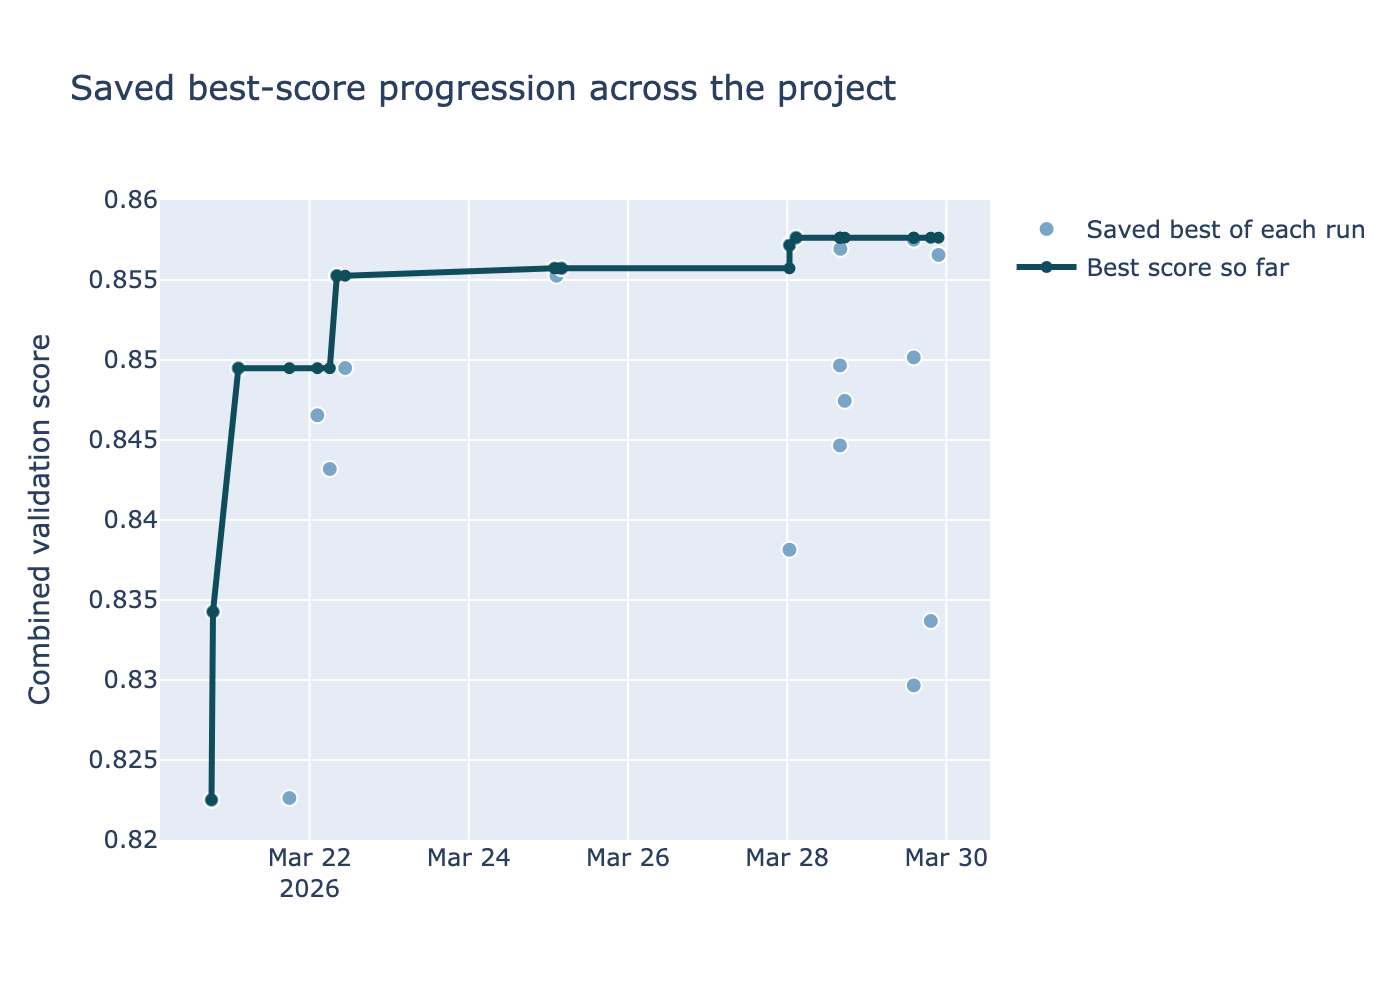
\includegraphics[width=\linewidth]{figures/methods_score_progression.png}
    \caption{Saved best-score progression across the project. The general pattern was steady upward motion, but the gains became smaller and more expensive late in the project.}
\end{figure}

\begin{figure}[H]
    \centering
    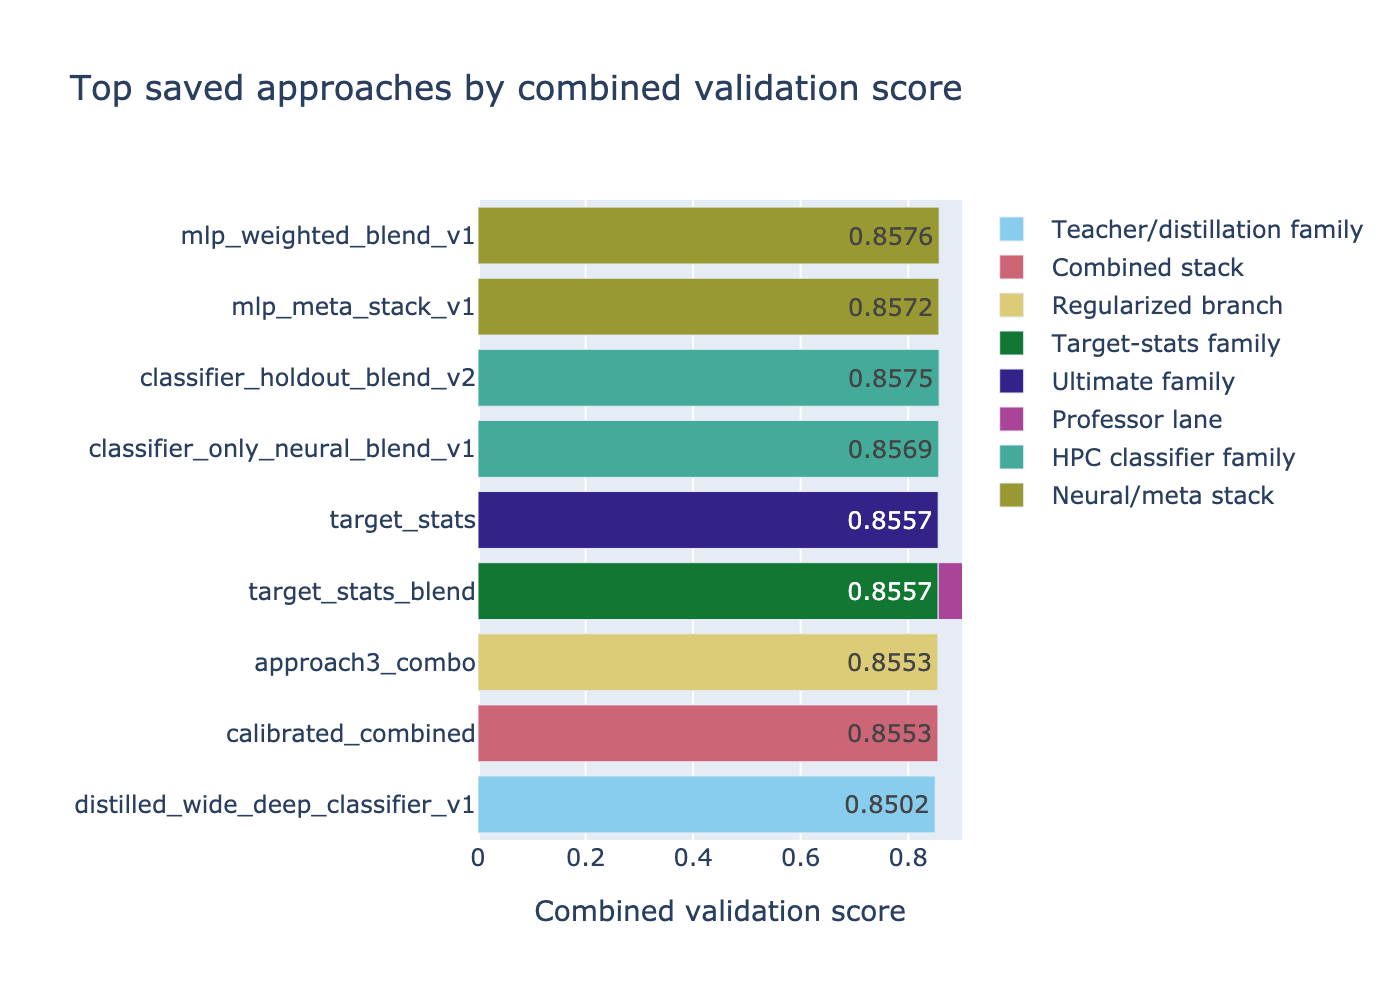
\includegraphics[width=\linewidth]{figures/methods_top_approaches.png}
    \caption{Top saved approaches by the combined validation metric. The strongest rows are not isolated single models; they are blends sitting on top of strong tabular sources.}
\end{figure}

Three takeaways kept repeating:

\begin{itemize}
    \item Stronger feature artifacts mattered more than cosmetic model swapping.
    \item The best local scores came from combinations of good branches, not from one heroic standalone model.
    \item The project improved when it stayed selective. The most expensive feature or model idea was not automatically the best one.
\end{itemize}

This is why the project eventually settled on a layered story: build a reliable tabular source first, then add a lighter combination layer on top if it earns its keep.
